\documentclass[a4paper,12pt]{book}
\usepackage[T1]{fontenc}
\usepackage[utf8]{inputenc}
\usepackage{lmodern}

%----------------------------------------------------------------------------------------
% Enlaces en las paginas y entre seciones
%----------------------------------------------------------------------------------------
\usepackage{comment}
\usepackage{url}
%\usepackage[breaklinks]{hyperref}
\usepackage{breakurl}




%----------------------------------------------------------------------------------------
% Colores
%----------------------------------------------------------------------------------------
\usepackage{xcolor} % Required for specifying colors by name
\definecolor{grey40}{RGB}{40,40,40} % Define the orange color used for highlighting throughout the book

%----------------------------------------------------------------------------------------
% Link a referencia
%----------------------------------------------------------------------------------------
%\usepackage[breaklinks]{hyperref}
\usepackage{hyperref}
\hypersetup{
   bookmarks=true,          % show bookmarks bar?
   pdftoolbar=true,         % show Acrobat’s toolbar?
   pdfmenubar=true,         % show Acrobat’s menu?
   pdffitwindow=false,      % window fit to page when opened
   pdfstartview={FitH},     % fits the width of the page to the window
   colorlinks=true,         % false: boxed links; true: colored links
   linkcolor=black,         % color of internal links (change box color with linkbordercolor)
   %citecolor=green,        % color of links to bibliography
   %filecolor=magenta,      % color of file links
   %urlcolor=cyan           % color of external links
}

%----------------------------------------------------------------------------------------
% figuras y subfiguras
%----------------------------------------------------------------------------------------
\usepackage{graphicx}
\usepackage{subcaption}


%----------------------------------------------------------------------------------------
% Bordes de las paginas
%----------------------------------------------------------------------------------------
\usepackage{geometry}
 \geometry{
 a4paper,
 total={170mm,257mm},
 left=20mm,
 top=20mm,
 }


%----------------------------------------------------------------------------------------
%	BIBLIOGRAPHY AND INDEX
%----------------------------------------------------------------------------------------

\usepackage[style=numeric,
            citestyle=numeric,
            sorting=nyt,
            sortcites=true,
            autopunct=true,
            babel=hyphen,
            hyperref=true,
            abbreviate=false,
            backref=true,
            backend=biber]{biblatex}
\addbibresource{bibliography.bib} % BibTeX bibliography file
\defbibheading{bibempty}{}


% pacote babel ou equivalent

\title{Humanismo Socio-político}
\author{Fernando Pujaico Rivera}

\begin{document}

\maketitle

\renewcommand*\contentsname{Conteúdo}
\tableofcontents

%----------------------------------------------------------------------------------------
%	PART
%----------------------------------------------------------------------------------------
\part{Explicación Part A}
\chapter{Desigualdad social }
\section{Tipos de igualdad jurídica}
\subsection{Igualdad ante la ley}
\subsection{Igualdad mediante la ley}

\section{Igualdad, equidad y justícia }
 Figura \ref{fig:DesigualdadSocial}

\begin{figure}[ht!]
    \centering
    \begin{subfigure}{0.3\textwidth}
        \caption{Igualdad.}
        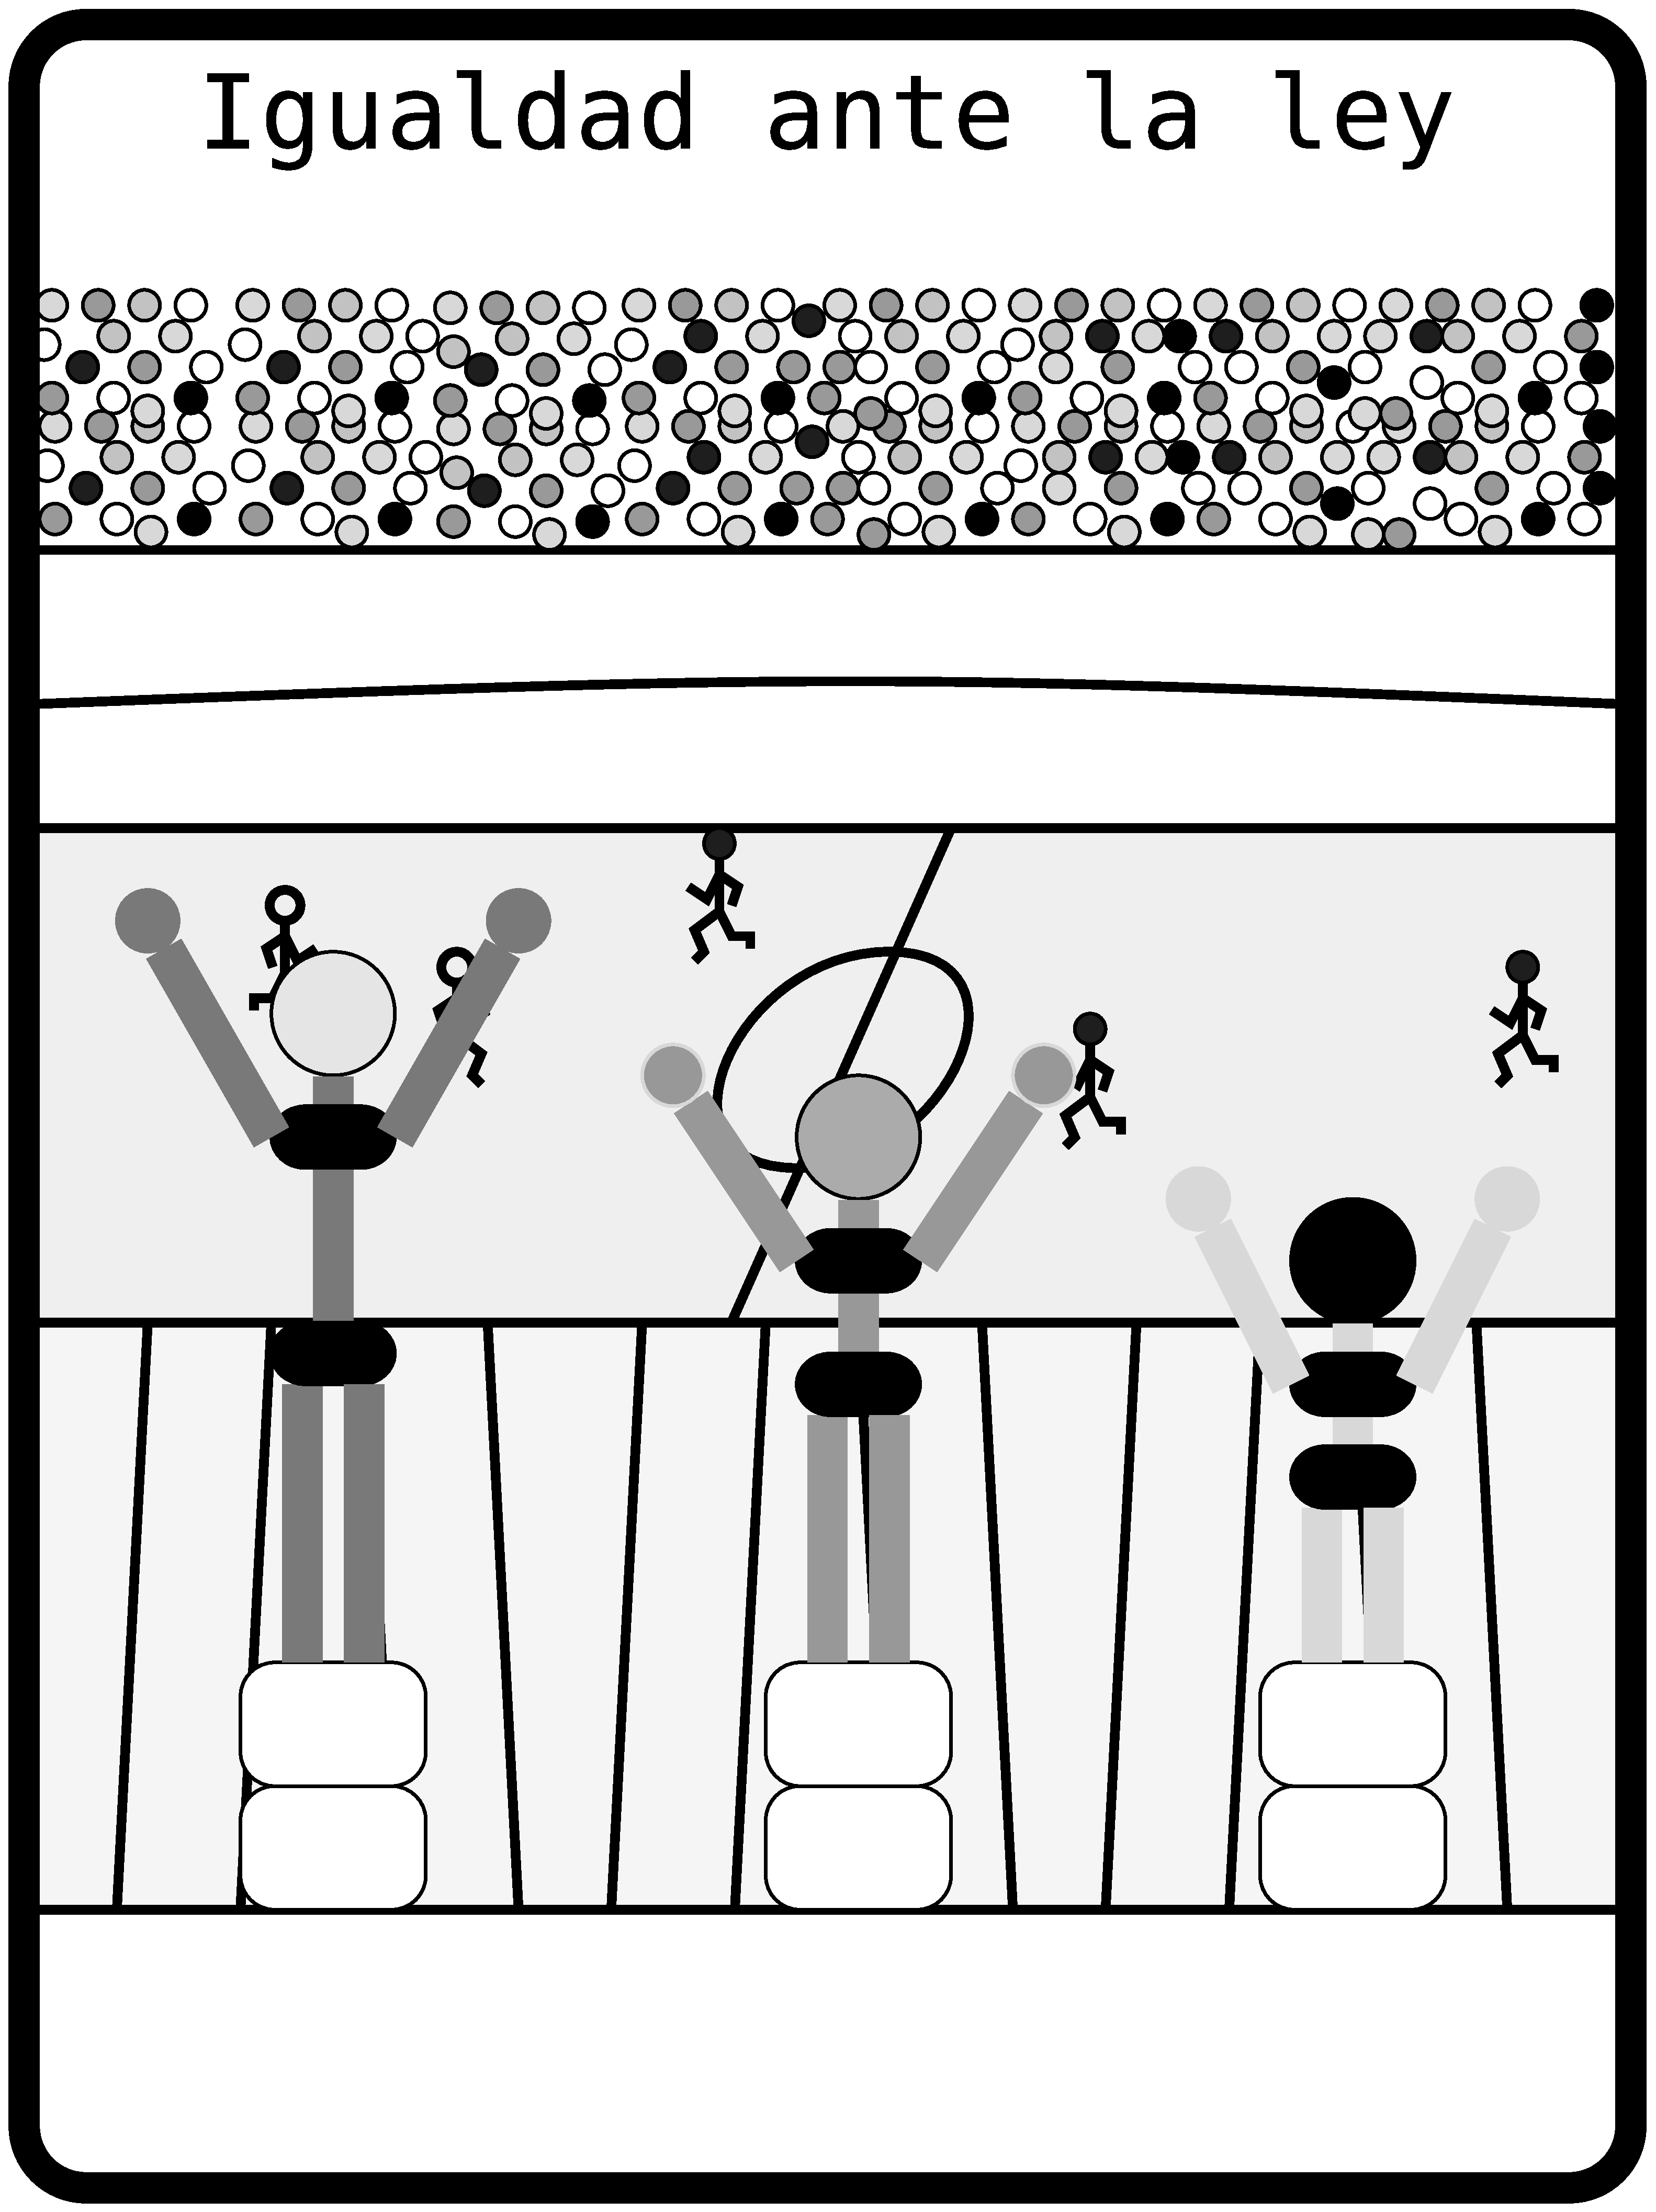
\includegraphics[width=\textwidth]{caps/desigualdad/igualdad.eps}
        \label{fig:igualdad}
    \end{subfigure}
    ~ %add desired spacing between images, e. g. ~, \quad, \qquad, \hfill etc. 
      %(or a blank line to force the subfigure onto a new line)
    \begin{subfigure}{0.3\textwidth}
        \caption{Equidad.}
        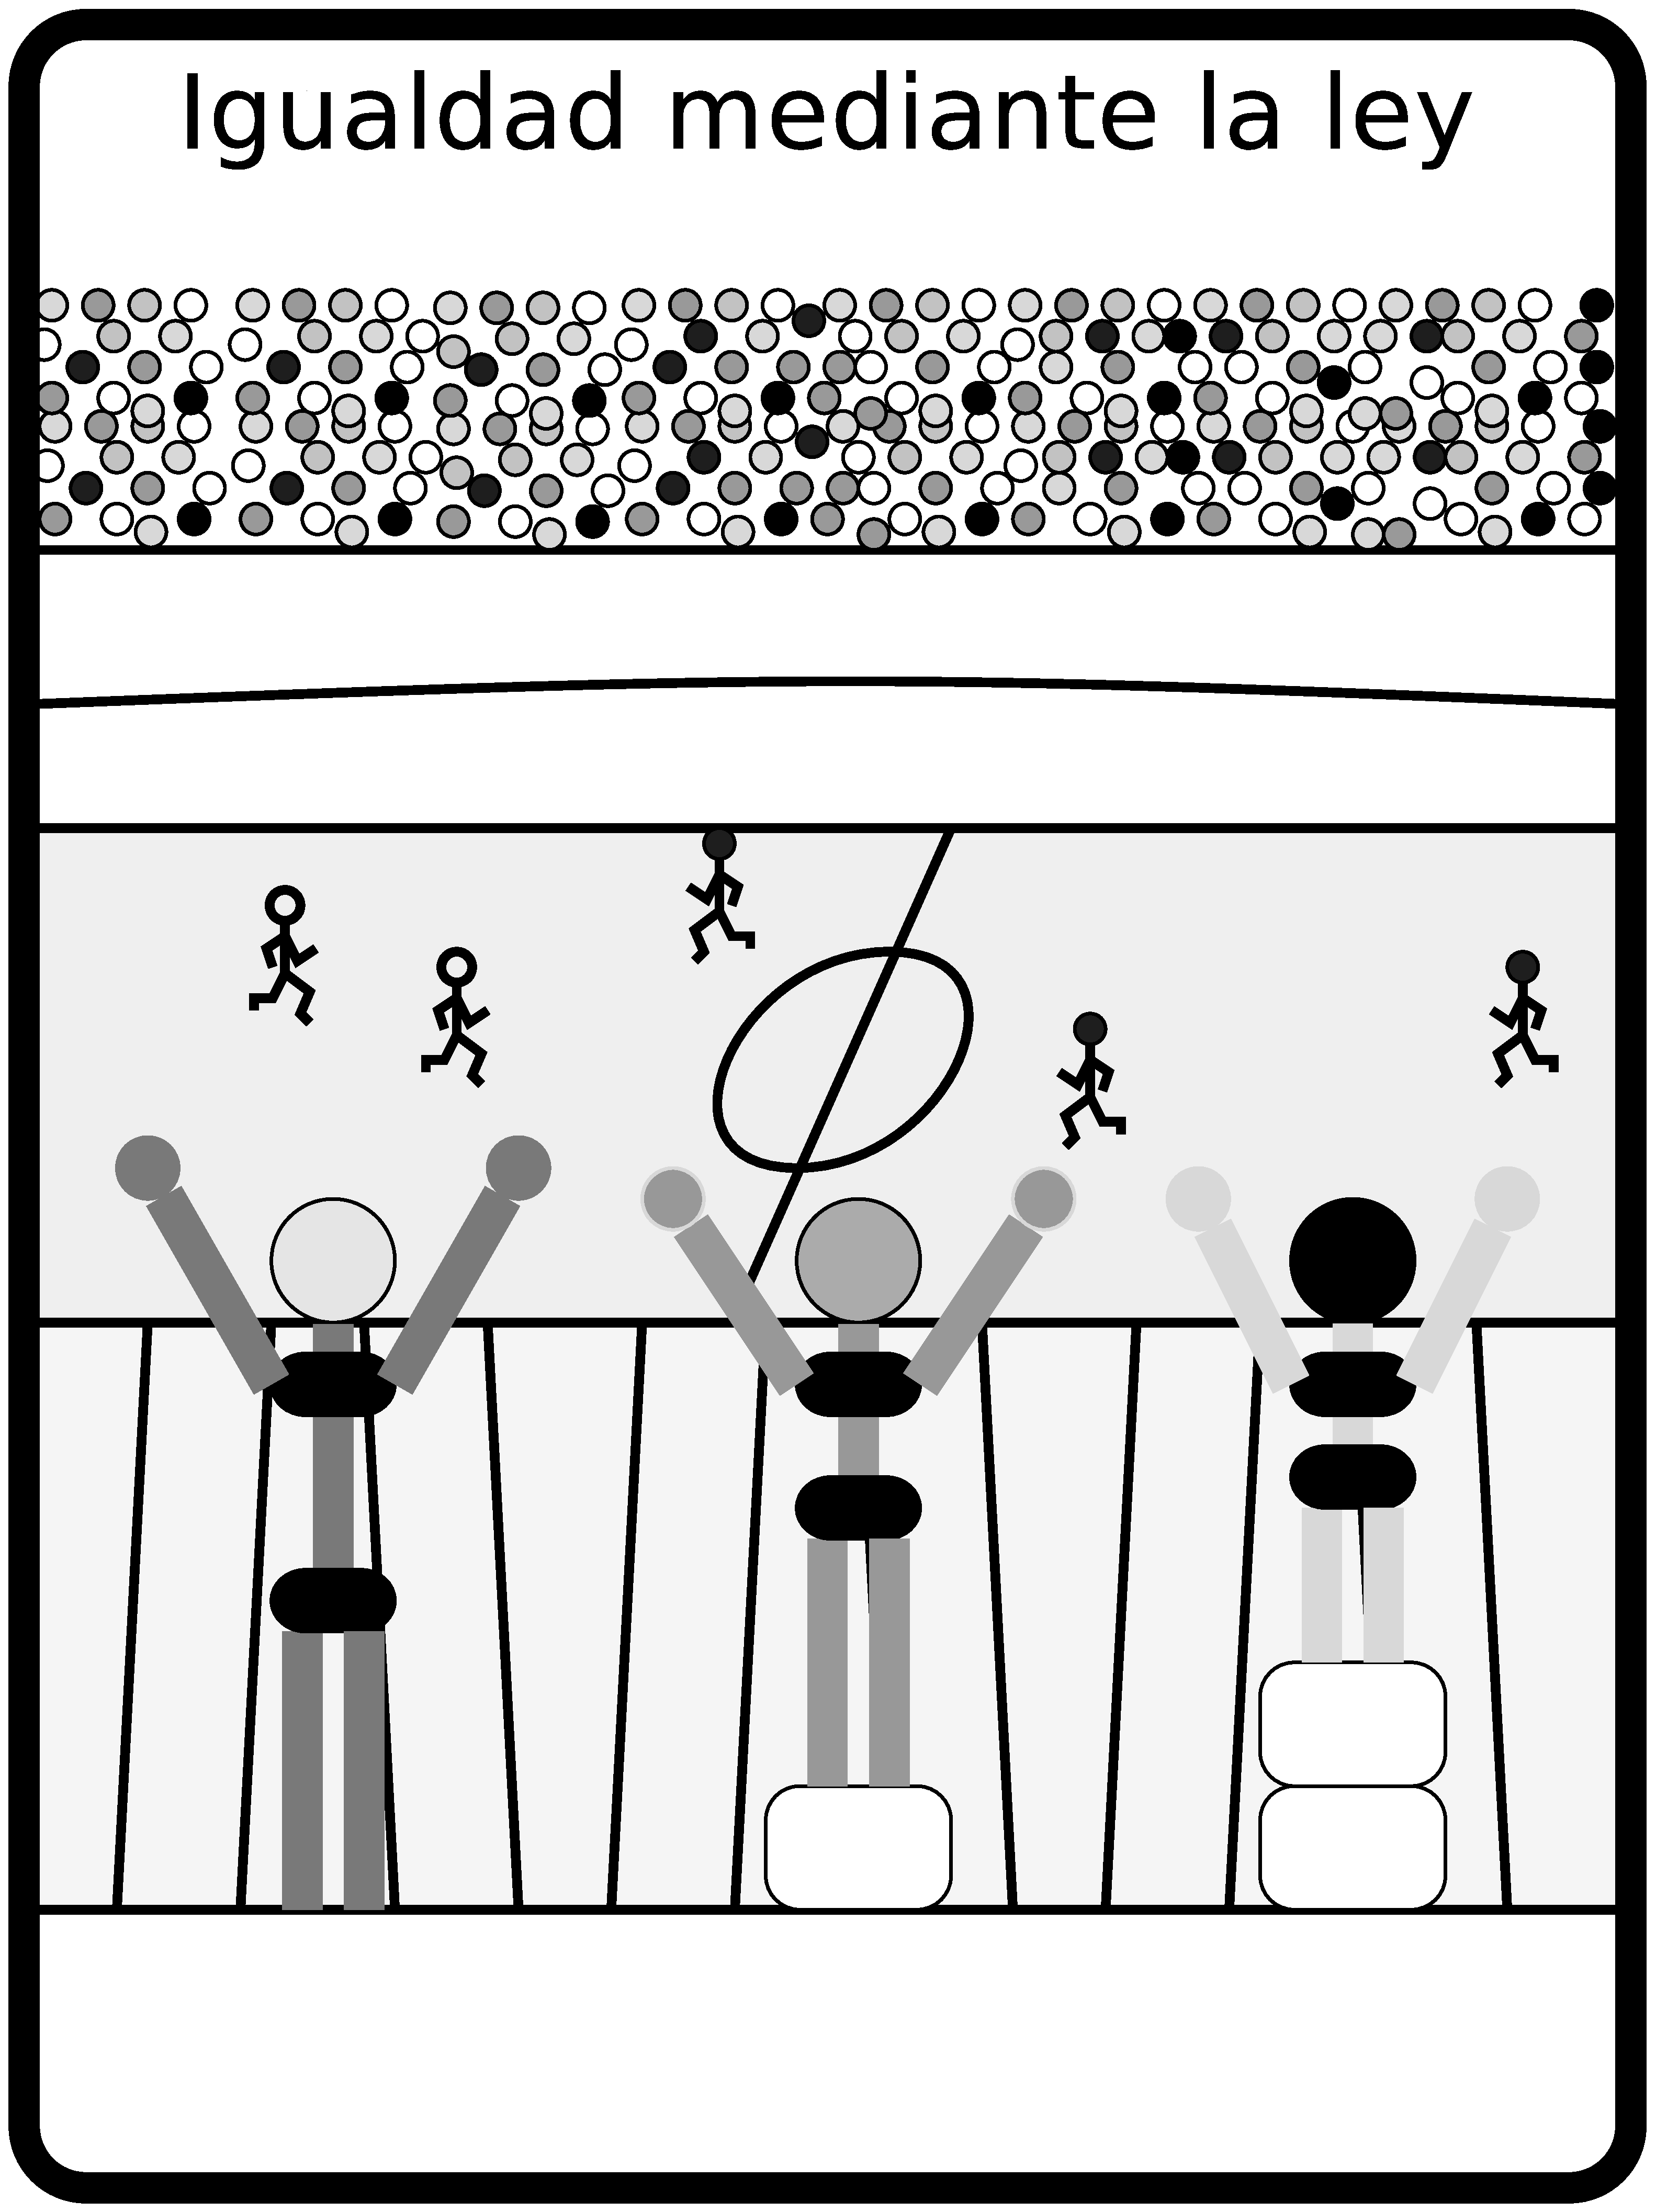
\includegraphics[width=\textwidth]{caps/desigualdad/equidad.eps}
        \label{fig:equidad}
    \end{subfigure}
    ~ %add desired spacing between images, e. g. ~, \quad, \qquad, \hfill etc. 
      %(or a blank line to force the subfigure onto a new line)
    \begin{subfigure}{0.3\textwidth}
        \caption{Justicia.}
        \includegraphics[width=\textwidth]{caps/desigualdad/justicia.eps}
        \label{fig:justicia}
    \end{subfigure}
    \caption{Desigualdad social.}\label{fig:DesigualdadSocial}
\end{figure}

\subsection{Igualdad}

El estado no genera riquesa, y tiene el trabajo de repartirla por igual a todos.
\subsection{Equidad}
El estado no genera riquesa, y tiene el trabajo de repartirla con equidad bajos su propia subjetividad.

Quien medirá la subjetividad de la desigualdad, con que criterio y con que autoridad.
\subsection{Justícia}
El estado no genera riquesa, Usa sus recursos pra crear un escenario que ayude a todos
independientemente de sus particularidades.


%----------------------------------------------------------------------------------------
%	PART
%----------------------------------------------------------------------------------------
\part{Explicación Part B}

%%%%%%%%%%%%%%%%%%%%%%%%%%%%%%%%%%%%%%%%%%%%%%%%%%%%%%%%%%%%%%%%%%%%%%%%%%%%%%%%
%%%%%%%%%%%%%%%%%%%%%%%%%%%%%%%%%%%%%%%%%%%%%%%%%%%%%%%%%%%%%%%%%%%%%%%%%%%%%%%%
\chapter{Bases }
\section{Presuncion de inocencia} 

\section{La privación de la libertad}
rehabilitación e reinserción, ou aislación. No es venganza.

\section{Delito no justifica delito}
Ejecutar a una persona porque le ha quitado la vida a otra es venganza, no justicia.

\subsection{Sobre la pena de muerte}


\section{Derecho a la vida} 

La Declaración Universal de Derechos Humanos  \cite{DUDH}

\subsection{Sobre el aborto en caso de violación}
\subsection{Sobre el aborto en caso de peligro de la madre}

%%%%%%%%%%%%%%%%%%%%%%%%%%%%%%%%%%%%%%%%%%%%%%%%%%%%%%%%%%%%%%%%%%%%%%%%%%%%%%%%
%%%%%%%%%%%%%%%%%%%%%%%%%%%%%%%%%%%%%%%%%%%%%%%%%%%%%%%%%%%%%%%%%%%%%%%%%%%%%%%%
\chapter{Violencia en la sociedad}

\section{Violencia intra-familiar} 

\section{Violencia en la pareja} 

\section{Violencia por discriminación} 
racista, sexista, por ideologia, genero, etc.

\section{Violencia social} 


\chapter{Anexos}

\section{Humanismo, Igualitarismo e Feminismo }


\section{Machismo e Hembrismo }




%----------------------------------------------------------------------------------------
%	BIBLIOGRAPHY
%----------------------------------------------------------------------------------------

\chapter*{Bibliografia}
\addcontentsline{toc}{chapter}{\textcolor{grey40}{Bibliografia}}
\printbibliography[heading=bibempty]


\end{document}
